\section{Subsystem Decomposition}
\label{sec:SubsystemDecomposition}

By dividing our system into smaller subsystems, the workload can be distributed among development teams and components that are already available to developers can be reused. The subsystems were identified by analyzing the flow of events shown in Figure \ref{fig:useCaseConsumer} and \ref{fig:useCaseProvider}. Each subsystem has precisely defined interfaces that are provided to its consumers and thus enable a modular architecture in which subsystems can easily be replaced by more efficient alternatives. Furthermore, our design enables implementations that support importing multiple IDL types and generating output for multiple programming languages at the same time. 

\begin{figure}[h]
	\centering{
		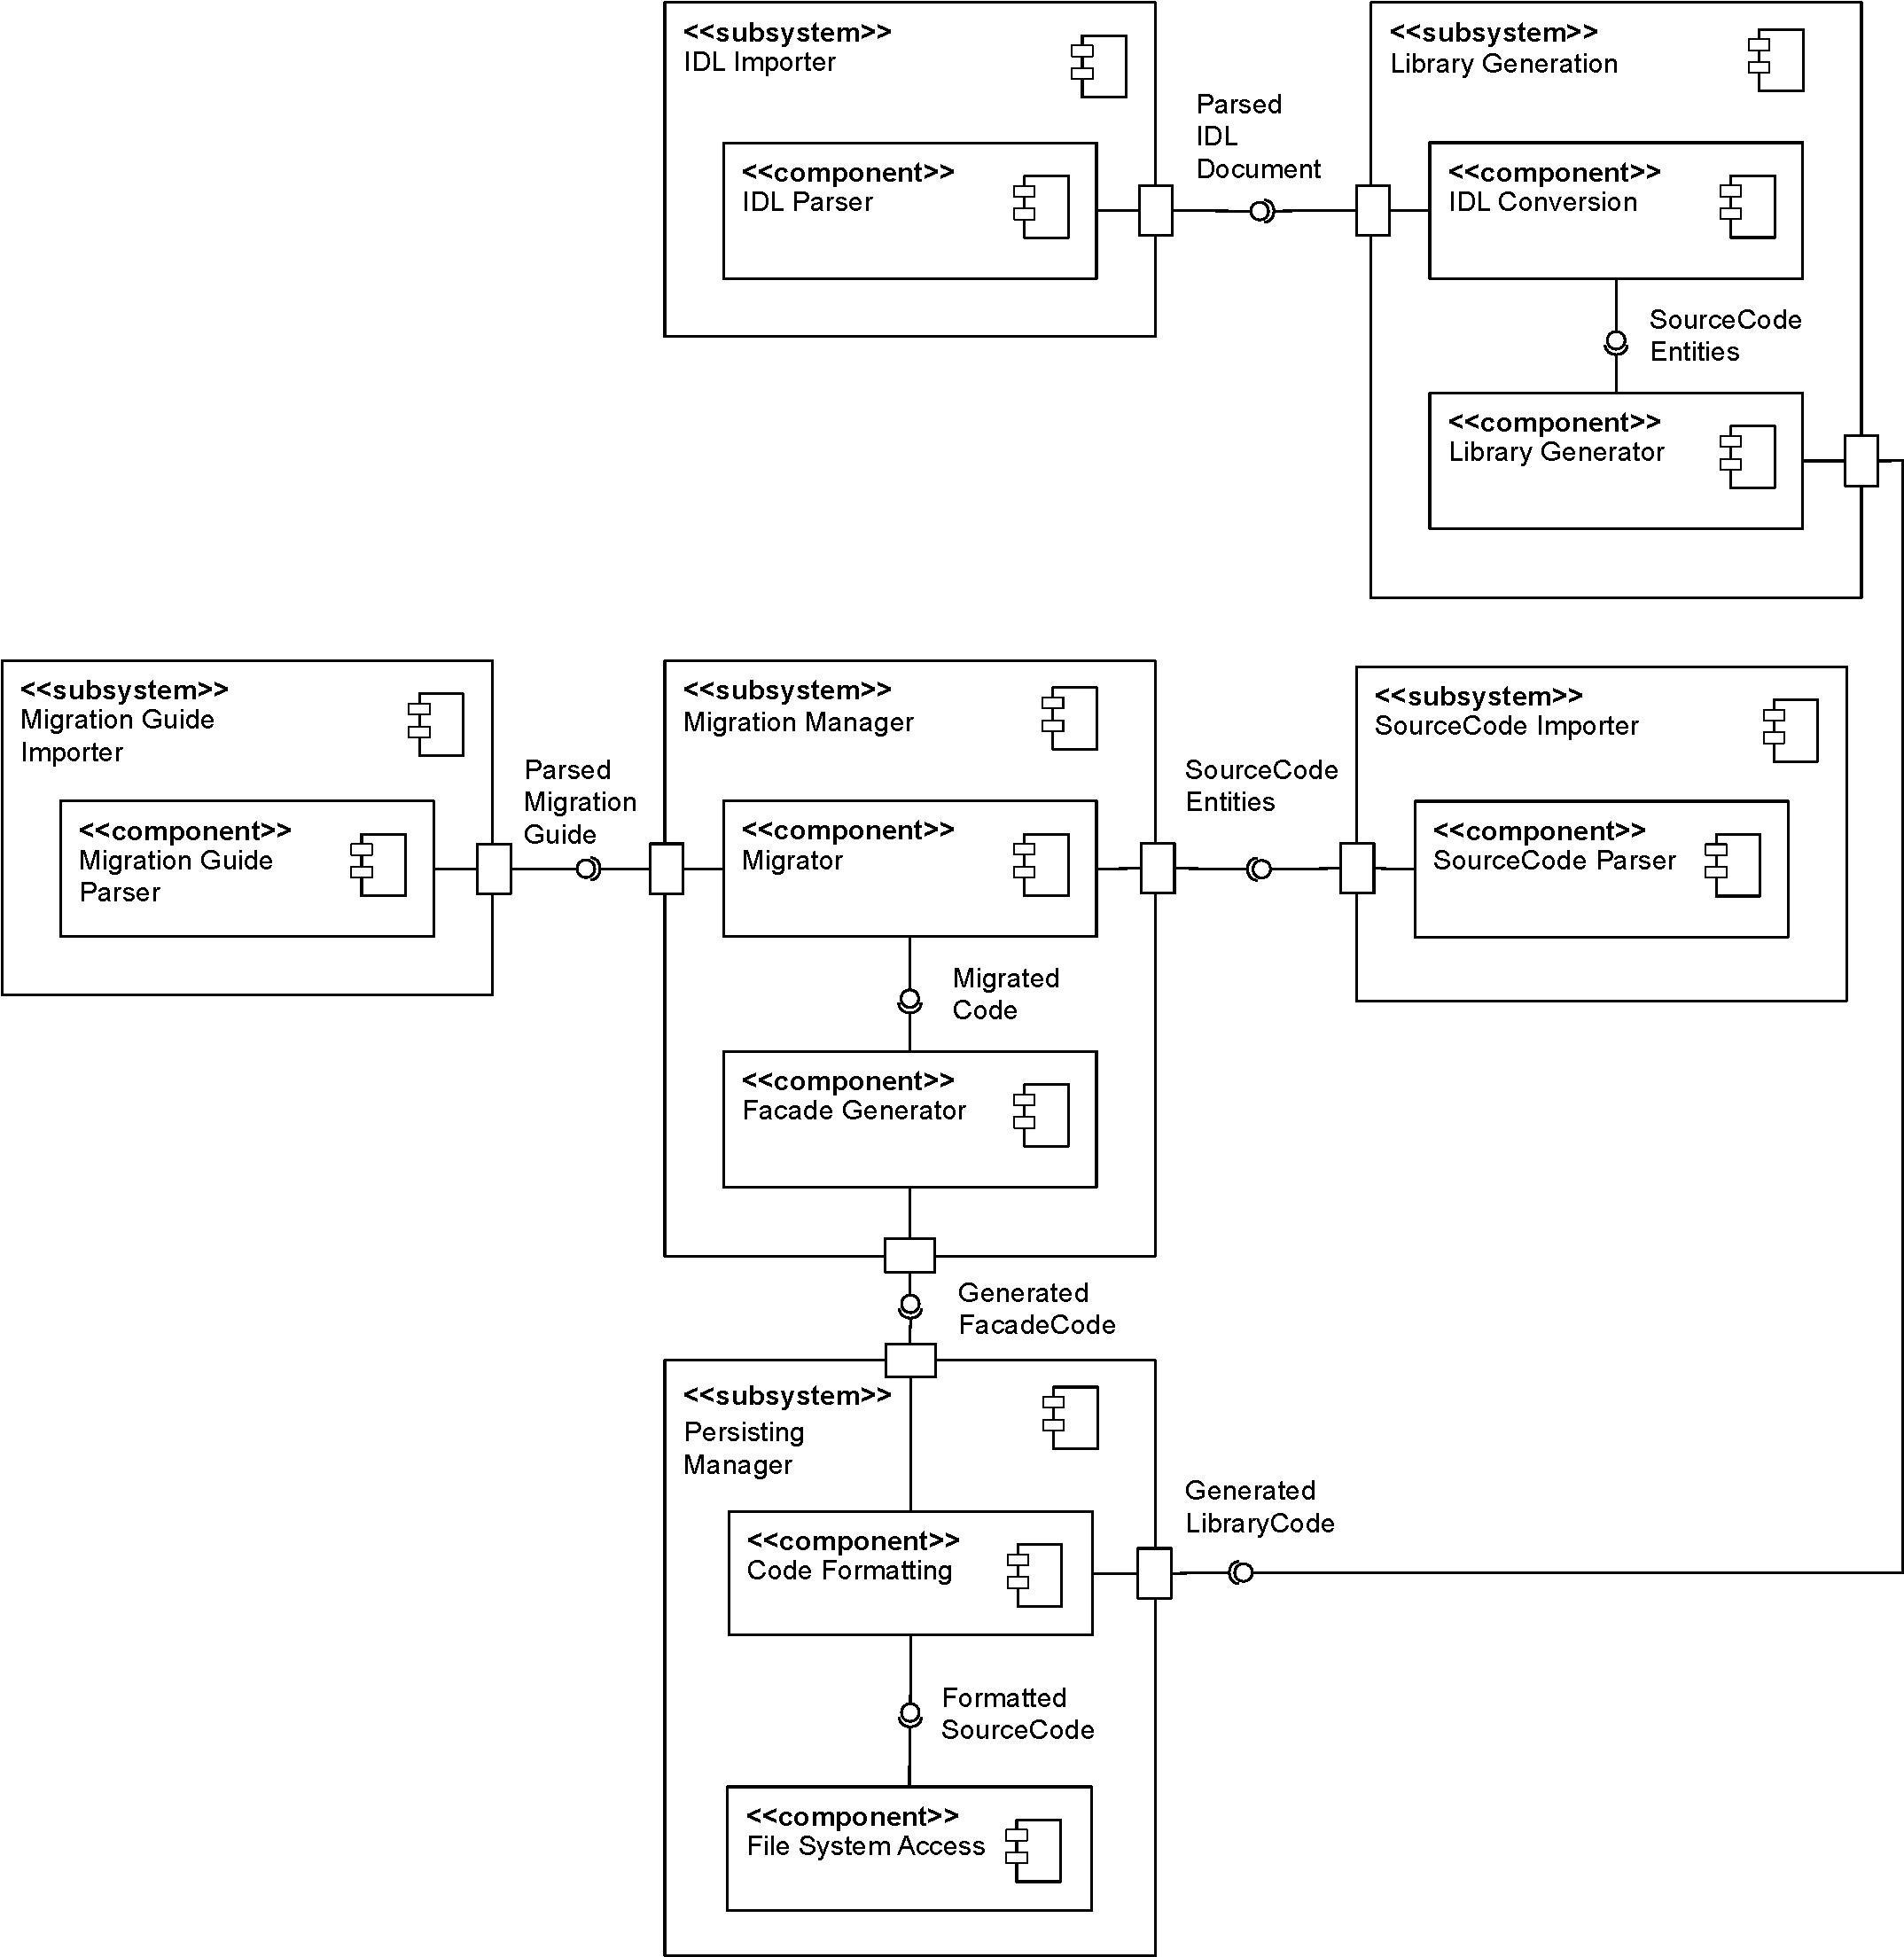
\includegraphics[width=155mm]{images/subsystem_decomposition.pdf}
		\caption{Subsystem decomposition}
		\label{fig:subsystemDecomposition}
	}
\end{figure}

For creating the library and persistent facade subsystem as shown in Figure \ref{fig:outcome}, various tasks need to be executed in order to generate them from IDL documents, previous versions of them and a machine-readable migration guide. 

In order to generate the library subsystem an IDL document must be imported and converted into the source code of a specific programming language. Therefore, a dedicated \texttt{IDL} \texttt{Importer} subsystem for reading and parsing of an IDL document supplies its encoded representation to the \texttt{Library} \texttt{Generation} subsystem. This converts the encoded IDL document into a textual representation of source code of a selected programming language. 

Creating the persistent facade subsystem requires the interaction of several resources that have to be imported first. Our migration guide as shown in Figure \ref{fig:migGuide} includes any changes made to the Web API between the previous and current versions. The corresponding \texttt{Migration} \texttt{Guide} \texttt{Importer} subsystem handles all of the tasks related to fetching, parsing, and validating a migration guide. It provides the parsed representation of the document to the \texttt{Migration} subsystem. For some types of changes, missing information is too cumbersome to be defined in a migration guide and cannot be implicitly derived from an IDL document. Therefore, the source code of the previous version of the facade subsystem must be analyzed to obtain this information. The \texttt{SourceCode} \texttt{Importer} subsystem reads and parses all files of the previous facade and library to provide the encoded result to the \texttt{Migration} subsystem. The \texttt{Migrator} component uses the received information to adapt the previous version of the facade using the changes as stated in the migration guide. Its output is used by the \texttt{Facade} \texttt{Generator} component to generate a textual representation of source code in the desired programming language. 

The emitted source code from both subsystems, \texttt{Migration} and \texttt{Library} \texttt{Gen\-er\-a\-tion}, is used by the \texttt{Persisting} \texttt{Manager} subsystem which formats the code according to a user-defined linting rule set. The formatted source code is written to file using the \texttt{File} \texttt{System} \texttt{Access} component.


